\section{\sysname~ Design}
\label{sec:design}

% Design goals:
%   A research platform
%     Easy to use, adjust source code, modification points
%     Full system stack: controller (load balancer), worker(s), load generation, containers, workloads, simulation
%     Configurable, lots of knobs to adjust things easily
%     Tracking of metrics/resources/system events
%   low-variance! and low(ish)-overhead platform
%   No frivilous features, not too complicated

\sysname's design is guided by our experience with OpenWhisk performance, and our goals of predictable performance, modularity, and providing a platform for reliable serverless computing research.

\subsection{Architecture and Overview}

The \sysname~ control plane is spread out across a load balancer and the individual workers.
We have found that most of the control plane overhead is in the workers, and hence optimizing the worker performance is our major focus.
We use stateless load-balancing, by using variants of consistent hashing with bounded loads (CH-BL), which have been proposed for FaaS recently~\cite{fuerst-hpdc23}.
This is a locality-aware scheme, which runs functions on the same servers to maximize warm starts, and forwards them to other servers only when the server's load exceeds some pre-specified load-bound.
Our architecture is thus \textbf{worker-centric}, and places more performance and load-management responsibility on the individual workers, instead of a more top-down centralized approach favoured by prior work such as Atoll~\cite{} and others Hermod/core-level~\cite{}. 
Top-down resource management requires a consistent global view of the cluster, and the predictive techniques commonly found in such architectures are complementary to our work.
%The worker-centric design allows us to find the limits of performance without making workload assumptions . 
Minimal and composable with other higher level cluster management (k8s etc), and also other isolation mechanisms.


\sysname's architecture is shown in Figure~\ref{fig:arch}.
Clients/users invoke functions using an HTTP or RPC API, with operations shown in Table~\ref{tab:api}. 
Continuing on the worker-centric theme, the worker API is a subset and almost completely identical to the overall API, and functions can be launched directly on a worker for single-worker setups and benchmarking, without going through a load-balancer and adding unnecessary latency.
The workers implement various latency-hiding and burst-mitigation techniques. 
All functions are launched inside containers, and dealing with the container layer is a major part of the worker. 
Each worker maintains a container pool of initialized containers for facilitating warm starts, and has an invocation queue for handling dynamic loads.
Invocation characteristics are captured in various datastructures and provided using APIs for developing data-driven resource management policies. 

%%%%%%%%%%%%%%%%%%%%%%%%%%%%%%%%%%%%%%%%


% \subsection{Function handling in the workers}

\subsection{Function lifecycle}

Function lifecycle is controlled by three main \sysname~ worker API calls.
New functions need to be first \emph{registered}, which entails downloading and preparing its container disk image.
The container images are downloaded from DockerHub or some other image repository.
Container images are composed of multiple copy-on-write layers, and we prepare the images by selecting the relevant layers for the operating system and CPU architecture.
\alex{IMPL: How's image created . HTTP server add etc.} 
%
Registered functions can then be directly \emph{invoked}, which triggers launching of the function's container. 
Each function container starts an HTTP server, which listens for and controls the actual function code execution.
\alex{Describe this http server API in the impl.}
When the container is ready, the worker sends an HTTP request to start the function code execution.
We detect the container's readiness using an inotify callback, which is a faster and more generic mechanism for notification compared to Docker's built-in API. 
%
%\alex{How do we know container is ready?}
Finally, when the function finishes execution, the HTTP call to the container's HTTP server returns, and the container is marked as  'available' in the container pool, to be potentially used for future invocations of the same function.


In the spirit of a fast ``baseline'' control plane and for isolation, \sysname~ does not share containers across functions.
For example, recently proposed optimizations allow for functions to share a language runtime inside a container~\cite{}. 

Additionally, \sysname~ introduces a standard \texttt{prewarm}  API call, which starts the function's container and the HTTP server inside of it, and adds it to the container pool.
This reduces most of the cold-start overhead associated with the container.
Prewarming can both avoid a "thundering herd" of cold starts on load startup, and be an optimization in which the control plane anticipates invocations and prepares containers for them. 
This allows for a systematic mechanism to implement various recently proposed predictive prewarm policies~\cite{zhou2022aquatope, icebreaker, shahrad,..}. 

\alex{Impl: prewarm, HTTP server imports python packages. Py specific opt}  

All of these steps contribute to our control plane overhead.
The total end to end latency, also called flow time is ...
The function code's execution time is the function;s wall-clock time after the agent executes it. It represents the baseline, ``best case'' performance without any FaaS overheads. 


\subsection{Worker Performance Optimizations}

\sysname~ workers use various resource management and implementation techniques to provide low latency function execution for heterogenenous and bursty workloads.

\noindent \textbf{Resource Caching.}
The cornerstone design goal of \sysname~ is to reduce jitter, which we accomplish by removing expensive operations from the function's critical path.
Instead, we pre-allocate as many function resources as possible, such as the container image, the container itself, network namespaces and virtual interfaces, etc.
\sysname~ maintains a cache all these resources, and the ``hot path'' function invocation latency is thus significantly lower than OpenWhisk, as we have shown earlier in Figure~\ref{fig:ow-ilu-overhead}.


\textbf{Network namespace caching.}
Each container requires network isolation, which we accomplish this by using network namespace provided by the kernel. 
These need not be created at the same time as the container they will isolate, letting us create a worker thread to maintain a pool of free network namespaces.
Moving this creation off the container creation critical path saves upwards of 100 milliseconds.

%Function registration triggers fetching the container disk image. 
%We also introduce a \texttt{prewarm} function action, which starts up the function's container (before it is actually invoked). 
%An invocation on the prewarmed container prevents a cold-start, and this allows us to implement many prewarming and pre-fetching policies like in~\cite{shahrad_serverless_2020}.

% \noindent \textbf{Disk image caching and pre-warming.}
% A \textit{cold start} occurs if a function is run on a worker that does not have a container available for it.
% This can be exacerbated if the worker has never seen that specific function previously.
% The latter case we handle by requiring a function to be \emph{registered} with the worker before invocation.
% Allowing us to prepare its code, disk image, or other dependencies ahead of time.
% Our worker API exposes the ability to prewarm functions on-demand on a worker.
% Prewarming can both avoid a "thundering herd" of cold starts on load startup, and be an optimization in which the control plane anticipates invocations and prepares containers for them.
% Solutions to these two issues have been explored by numerous works~\cite{shahrad_serverless_2020}, and our design is extensible enough to support any of them. 




\noindent \textbf{Async function life-cycle handling.}
The second key design principle is to handle various aspects of the function's lifecycle asynchronously off the critical path. 
One such aspect is maintaining the function keep-alive cache, and ensuring that new functions have enough free memory to launch without waiting on existing containers to be evicted first.  
The container eviction from the keep-alive pool is done periodically in the background, similar to the Linux kernel page-cache implementation.
We maintain a memory buffer for dealing with invocation bursts, periodically sort the containers list for eviction based on caching policies from~\cite{faascache-asplos21}, and evict containers from the keep-alive pool.

\sysname~ workers maintain a queue of invocations instead of executing all functions synchronously; unlike existing popular FaaS control planes.
This allows us to spread the load of function bursts over time and reduce the maximum load and lock contention overheads.
In our experience, function bursts are the primary contributor of high control plane overheads, and mitigating them is a major challenge. 


\textbf{Evicting containers.}
In the event there is not enough memory on the server to cold-start and run a function, cached containers must be evicted to make room.
Traditionally eviction decisions would be made in an online fashion, but picking victims and waiting for their removal creates high variance in function execution times.
We alleviate this by proactively computing eviction priorities and maintaining a memory buffer for bursts of invocations. 
A thread routinely monitors all cached containers, ordering them based on an eviction algorithm, and, if necessary, removes some to maintain the bubble.

\textbf{Support for queuing policies.}
In serverless when any worker becomes overloaded, with either insufficient CPU or memory resources, it faces a choice.
New invocations can be dropped or they can be enqueued hoping for the load to lift.
\sysname{} workers support both modes of operation.
The latter case is more interesting, where we place all arriving invocations into a work queue that is monitored.
When resources are plentiful, they are started immediately and there is no latency impact.
Invocations are left queued when the system is under contstraint, our design leaves the possibility of re-ordering work while in the queue.
This allows for more advanced policies than the strict FIFO queue that other systems support.




\begin{comment}
  
\noindent \textbf{Networking.}
Similarly, other container startup operations such as creating network namespaces and virtual interfaces are also time-consuming.
\sysname~ both pre-allocates and caches them, saving more than 100s milliseconds in latency overhead.

We use CNI for using network bridges for 

Network namespaces are important for isolation.
But creating them is timeconsuming.
Our experiments found that more than 100ms can be spent on it by Linux. 
We use \textbf{network namespace caching} to get around this. 
We pre-create a large number of networking namespaces, and use them instead of creating new ones synchronously. 

Again, more networking solutions such as photon may be possible, but we wanted to investigate FaaS performance in the most general/default conditions.
\end{comment}

\begin{comment}
Mix of lightweight and heavy functions, so mix of simple request/microservice scheduling and ``packing''.
1. Keep the controller small and lightweight. Too much traffic to handle.
Locality is key, so assigning functions to their ``home'' servers is key.
Overloads are common and need multiple ways of mitigation:
1. CH-BL forwarding. 
2. Function queue on each worker/server. This has many other benefits  as explained in the next section.
3. \textbf{Workers responsible for most of resource management}. Centralized core-allocation unrealistic and unnecessary. The scale means that centralized  solutions can become untenable. Even partitioning cluster like atoll 
4. Ofcourse elastic scaling for workload dynamics. 


For a research platform: need solid simple APIs and real-time function information for data-driven policies.
Also be very simple. The worker and main controller API is nearly identical, so worker can be run standalone and optimizations can be developed using it. 


For \textbf{predictable latency}: move things away from the critical path and resource caching. 


\textbf{Find the limits of container orchestration.} 

Modular and \textbf{reactive}. Bare minimum functionality to see how far the boundaries can be pushed. Predictive techniques are good but complementary.
Also performance with predictive techniques depends heavily on workloads. The Azure trace is regular and large gains can be obtained with simple predictions and hard to make prediction-based systems like Atoll/Aquatope to be robust, general, and applicable in other real-world scenarios. Avoid overfitting or overoptimizing based on one trace. 

\end{comment}

\subsection{Containerization}

Multiple backends. By default, containerd. Also Docker.
Tradeoffs.
Finally, a ``null'' simulation backend for ...

We use containerd. Will be useful to say what the layers are: Docker, containerd, runc.
We get the container, image, namespace, and snapshot abstractions.
There is a tradeoff here: the container creation overheads can also vary significantly. The C implementation crun is 150ms, and runc is 200ms, containerd is 300ms, and docker is 350ms. This primarily affects the cold-start times. This is thus an important optimization opportunity for work on reducing cold-start times.

Container creation also requiring lots of process forks, which itself is few ms. One way to optimize this is to use \textbf{large pages.}


Pure rust-based implementation also possible. Part of future work. But also wanted to investigate and tackle the challenge of getting predictable performance out of higher level containerization services that are not part of the same address space.

We could have shaved off a lot more container overhead with our own containerization layer in the address-space instead of an external service like containerd. Avoid IPC and  extra communication in creating containers, tasks, etc. Reduce system calls and forks, and interface with the OS more directly and use optimizations for cgroups and namespaces that functions enable, compared to general purpose containers.
But doing so would make it hard to focus on the control plane. It is part of future work. 
%What aoptimizations could we do with a native containerization layer? Avoid IPC?

\textbf{We also have a docker backend?}

Including a ``null'' backend for examining just the control plane overheads and for simulation.

Previous FaaS system designs have focused on minimizing or eliminating container cold starts from their platform.
They remain an open issue, but we must be aware that the overwhwelming majority of invocations are warm hits.
A research platform must cater to this reality, while easily enabling various research avenues, including cold starts.

Using cgroups quotas? quota === cpus. period is 1 second. % This is correct. 
% https://github.iu.edu/prateeks/efaas/blob/f2a076055038fed7f99d9867b68427401e1f442e/src/Il%C3%BAvatar/il%C3%BAvatar_worker_library/src/services/containers/containerd/containerdlife.rs#L97



Once the container is created after modifying its container-spec (resource limits and disk image), a task launch actually starts running processes inside of it. Thus its a 2 step process. 

A major task is reading the image snapshot to find the base. \textbf{ZFS stuff?}


Finally, a major question is, why use OS containers for functions?
There has been an explosive growth in the number of sandboxing abstractions for serverless computing.
Lightweight VMs use stripped-down specialized hypervisors for reducing the ``boot time'' of functions, and are popular because they can provide additional isolation.
\sysname can work with these lightweight VMs such as Firecracker, since it is a containerd backend, and as a control-plane, it really does not focus on the isolation backend.

Resuming from some kind of a snapshot, like in Catalyzer, vhive, etc., is also a common technique for reducing the cold-start latency.
And finally isolation can be provided by language runtimes, such as WASM or graalVM.

These different isolation methods again mainly influence the cold-start times, and the other control plane operations remain unaffected. Exploring their performance is part of our future work.
We chose containers because they allow the shortest path to deploying FaaS, especially in private clusters, such as Funcx. 


or using other kinds of translation and interposition like in gVisor.

%%%%%%%%%%%%%%%%%%%%%%%%%%%%%%%%%%%%


%%%%%%%%%%%%%%%%%%%%%%%%%%%%%%

\subsection{Function Performance Model and Metrics}
Flow time = control plane overhead + queue time + processing time.

The control plane overhead depends on a lot of components such as the sandboxing layer etc.
The processing time is also dependent on system conditions and load, especially in overcommited scenarios.
Also because of the poor locality of function execution, this processing time can vary based on the concurrency level.


\begin{figure} 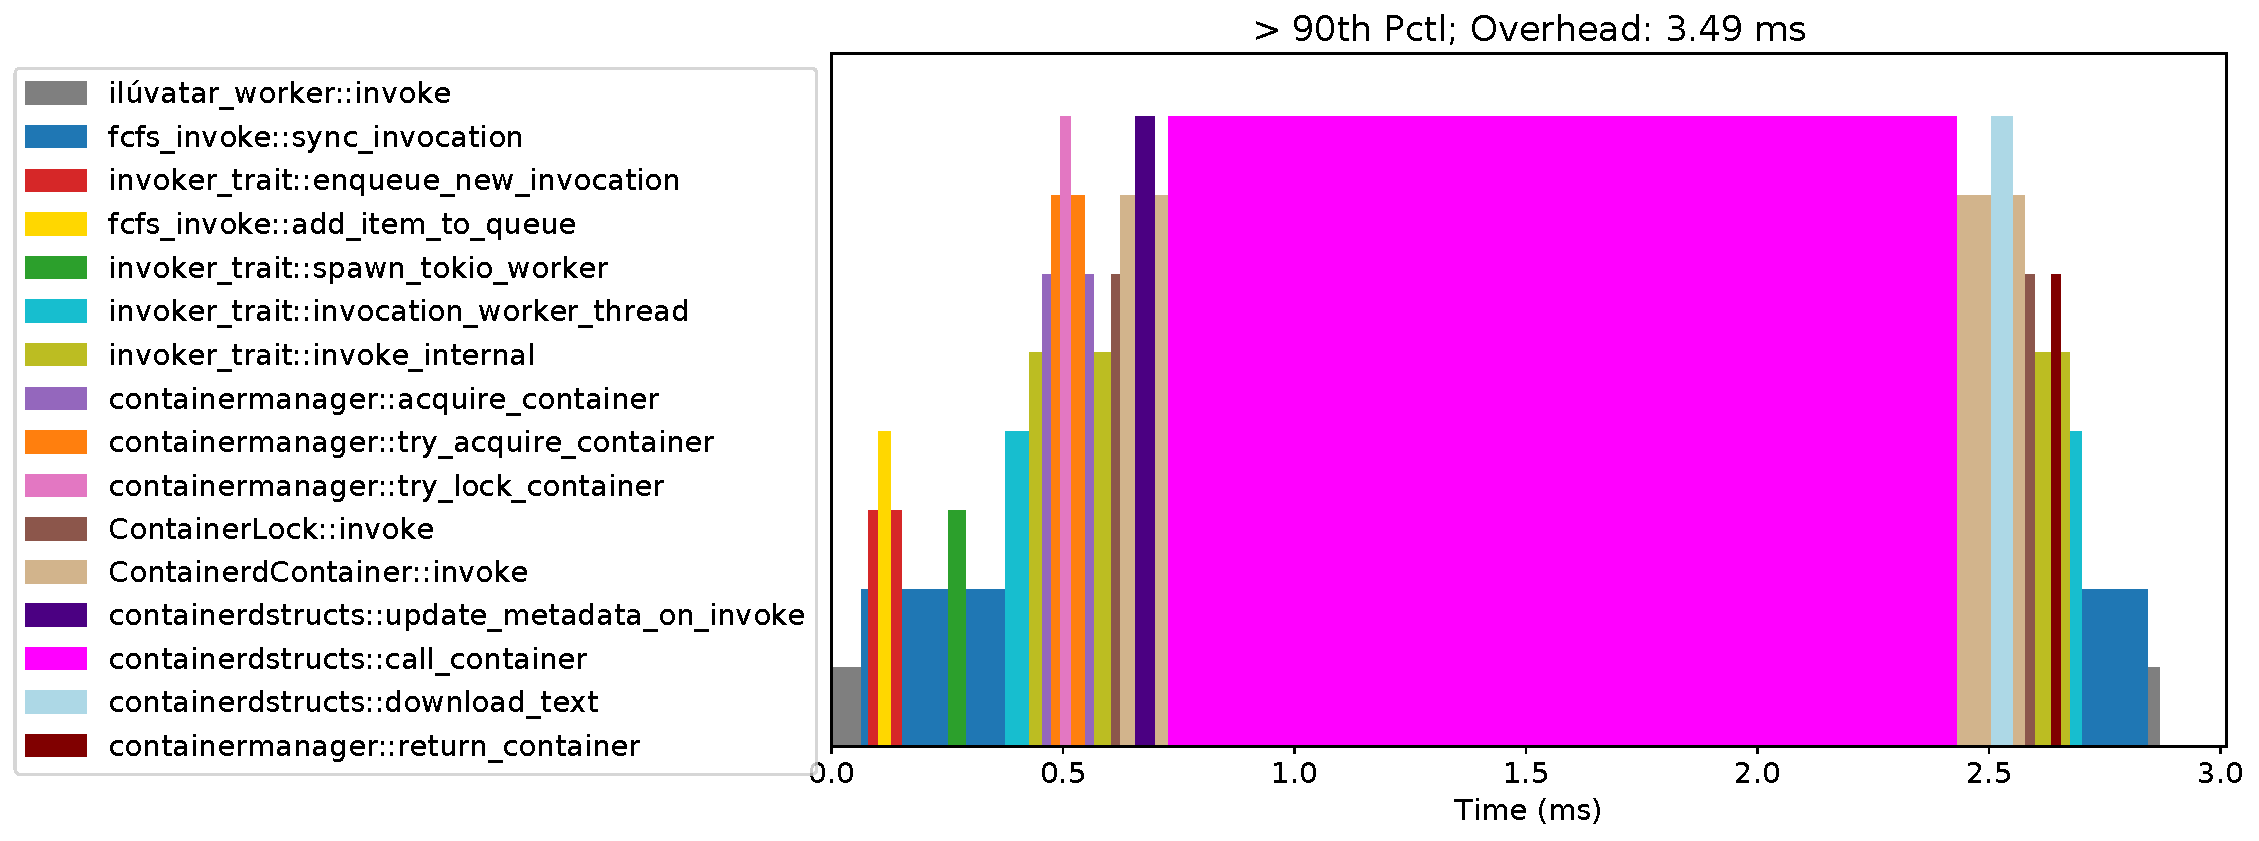
\includegraphics[width=\columnwidth]{../graphs/timelines/0-e1bc39-timeline.pdf}
    \caption{TODO: system diagram for The \sysname{} research platform.}
\end{figure}


\begin{comment}
\subsection{Main Components}

Two main parts: controller and worker.
Controller manages a pool of servers and performance functions like load-balancing and the endpoint for users to interface with the FaaS system and run functions.

The worker daemon runs on each server and forms the bulk of the control plane for running the functions.


\textbf{Controller.}

\subsection{Worker Operations}

Worker is assigned functions to run via the RPC API.
Either the controller for multi-server deployments, but also has the same API for standalone deployments and testing the performance in single-server setups, like function scheduling, keep-alive, etc. Not having the controller removes one additional component of jitter and simplifies the software stack.

Worker API is simple and minimalistic: invoke, invoke-async, prewarm, register, and status tracking using ping, status, health. 

Two-step process for reducing work on critical path.
\textbf{Prewarm} and
\textbf{Register} operation creates the container disk image and makes the function ``ready'' for execution. This removes a lot of cold-start overheads associated with fetching and building the image, and often takes around .... seconds.



Key structure is the container pool: list of running and warm containers for each function.


State Map ; characteristics map ; container pool

\end{comment}

\subsection{Other}


Our primary design consideration for \sysname{} was to make an easy to use, simple, complete, and useful research platform.
We designed the full system stack to allow for experimenting with any and all portions of the FaaS ecosystem.

The most complex piece of serverless stacks, and the focus of much previous work, is the \textbf{worker}.
Our worker runs on a single host server, and is responsible for execution function invocations.
To accomplish this, it performs a number of tasks:
\begin{enumerate}
    \item A function's code must be prepared by the worker.
    \item Proper isolation from other functions via some containerization scheme.
    \item Limiting concurrency to ensure system resources are not overwhwelmed.
    \item Evicting stale containers to free up memory and create new containers.
\end{enumerate}

As \sysname{} isn't a one-use research design, it must be extensible to future tinkering.
We imaging the worker supporting a variety of execution methods.
Classically FaaS has been CPU-based isolation, but there is great opportunity for enabling GPU, TPU, FPGA, and SmartNIC accelerator support.
We have designed the worker such that it can support multiple modes of function execution.
Something about this being future work...

While a single server is interesting, FaaS is a cloud offering that uses clusters of machines.
This requires a \textbf{controller} to act as an entrypoint to a cluster setup and to load balance invocations.
In addition, if a worker suffers a failure invocations must be re-directed to other workers.
The controller is expectedly simple, but in it's role can enable a variety of different load balancing policies.
Worker load, their execution capabilities, locality, cache availability, the controller can track all of these to improve the system.
% It's primary functions are to inform connected workers to new functions that are added to the system, and to try and keep any worker from having too much load to the detriment of user latency.

Load Generation: \textbf{Move to the evaluation section.} 


\subsection{Simulation backend}

As a complement in-situ experiments, many people perform simulations modeling their proposals.
These often differ wildly from live results, given that such a simulator is a different implementation.

We have designed \sysname{} such that it can run as a live system \emph{or as a simulation}, using exactly the same source code.
Thus an experiment can be run in-situ or in-silico, following identical code paths.
The only distinction is that network calls are replaced with function calls and function invocations are converted to sleep statements.

The final, and possibly the most important, part of a system to be used for research is exporting results and digging into them.
The major events of an invocation are recorded, and its details such as wall time and if it was a cold start can be returned to the client.
All the major components report and log metrics which can both inform online decisions, but allow offline analysis.


% \begin{enumerate}
%     \item A \textbf{controller} to act as an entrypoint to a cluster setup and to load balance invocations.
%     \item A \textbf{worker} that executes functions on a server, that can run standalone or as a cluster.
%     \item Several \textbf{containerization} backends that are both examples and efficient, usable implementations.
%     \item An open-load \textbf{load generator} that can apply arbitrary loads to our controller or worker.
%     \item \textbf{Workload synthesis} providing characteristics matching that of real-world FaaS workloads.
%     \item Benchmark \textbf{functions} adapted from FunctionBench~\cite{}, these track execution data for post-processing. 
%     \item A one-to-one \textbf{simulator} implementation of the controller and worker for fast prototyping and scalable testing.
%     \item \textbf{Logging} and recording of system events, metrics, and invocation statistics to allow for advanced post-processing.
%     \item Easy \textbf{Deployment} of \sysname{} via Ansible for simple orchestration. % - moved to impl
% \end{enumerate}

First and foremost, we put emphasis on having all pieces be low-overhead ($\sim$ 3 ms) and \emph{low-variance} on the invocation pipeline.


\begin{figure}
    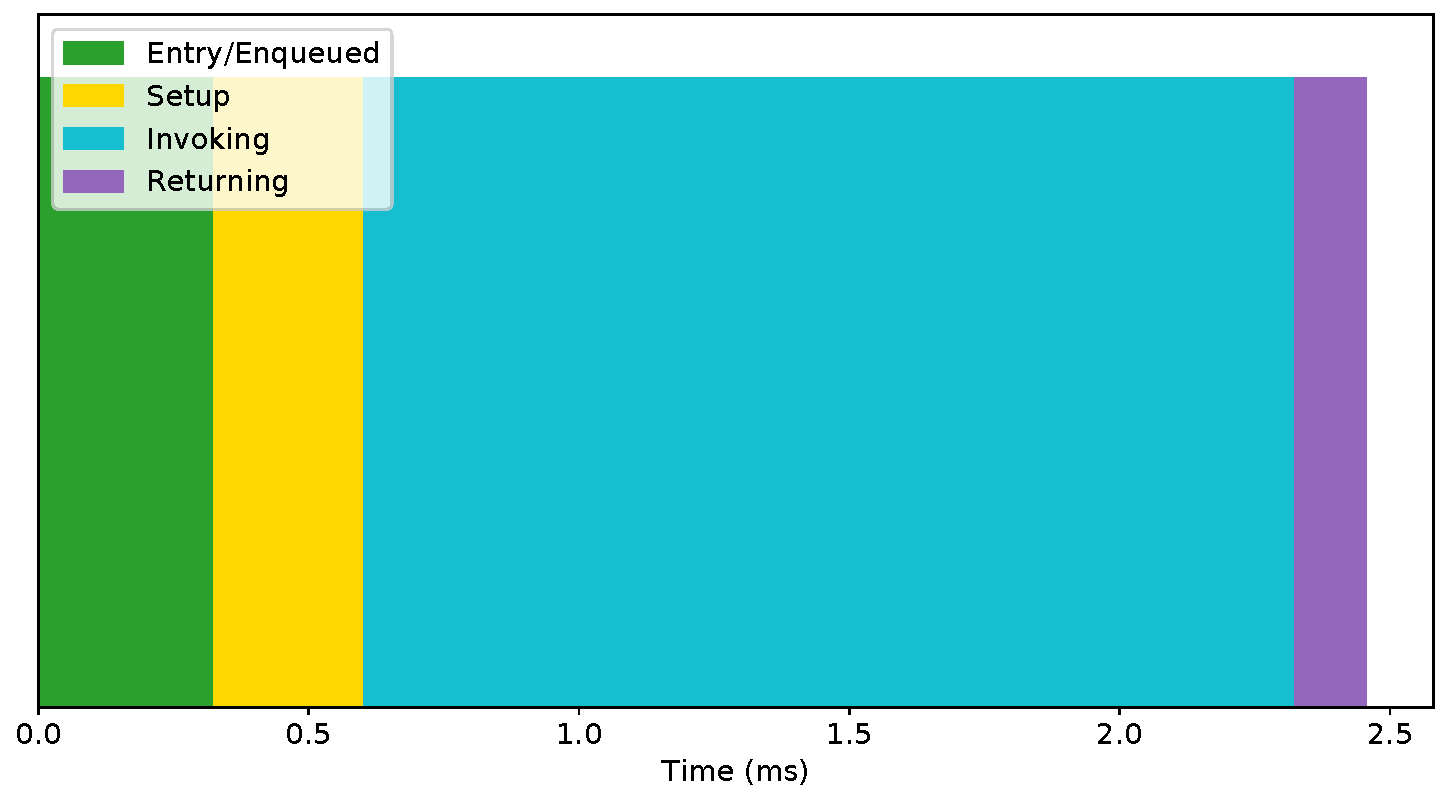
\includegraphics[width=\columnwidth]{../graphs/timelines/1-625b2e-simple-timeline.pdf}
    \caption{Timeline of the \sysname{} worker's overhead during a warm invocation.}
\end{figure}


\subsection{Other aspects}
Lastly, the \emph{tracing} crate enables us to capture spans of Rust function calls, especially entry and exit times, durations, and even parameters.
This logging enhances our ability to monitor the control plane overhead for better attribution of power usage.


%%% Local Variables:
%%% mode: latex
%%% TeX-master: "paper"
%%% End:
